\chapter{\label{method}Extensions and Innovation}
\section{With Iron}
\begin{figure}
	\centering
	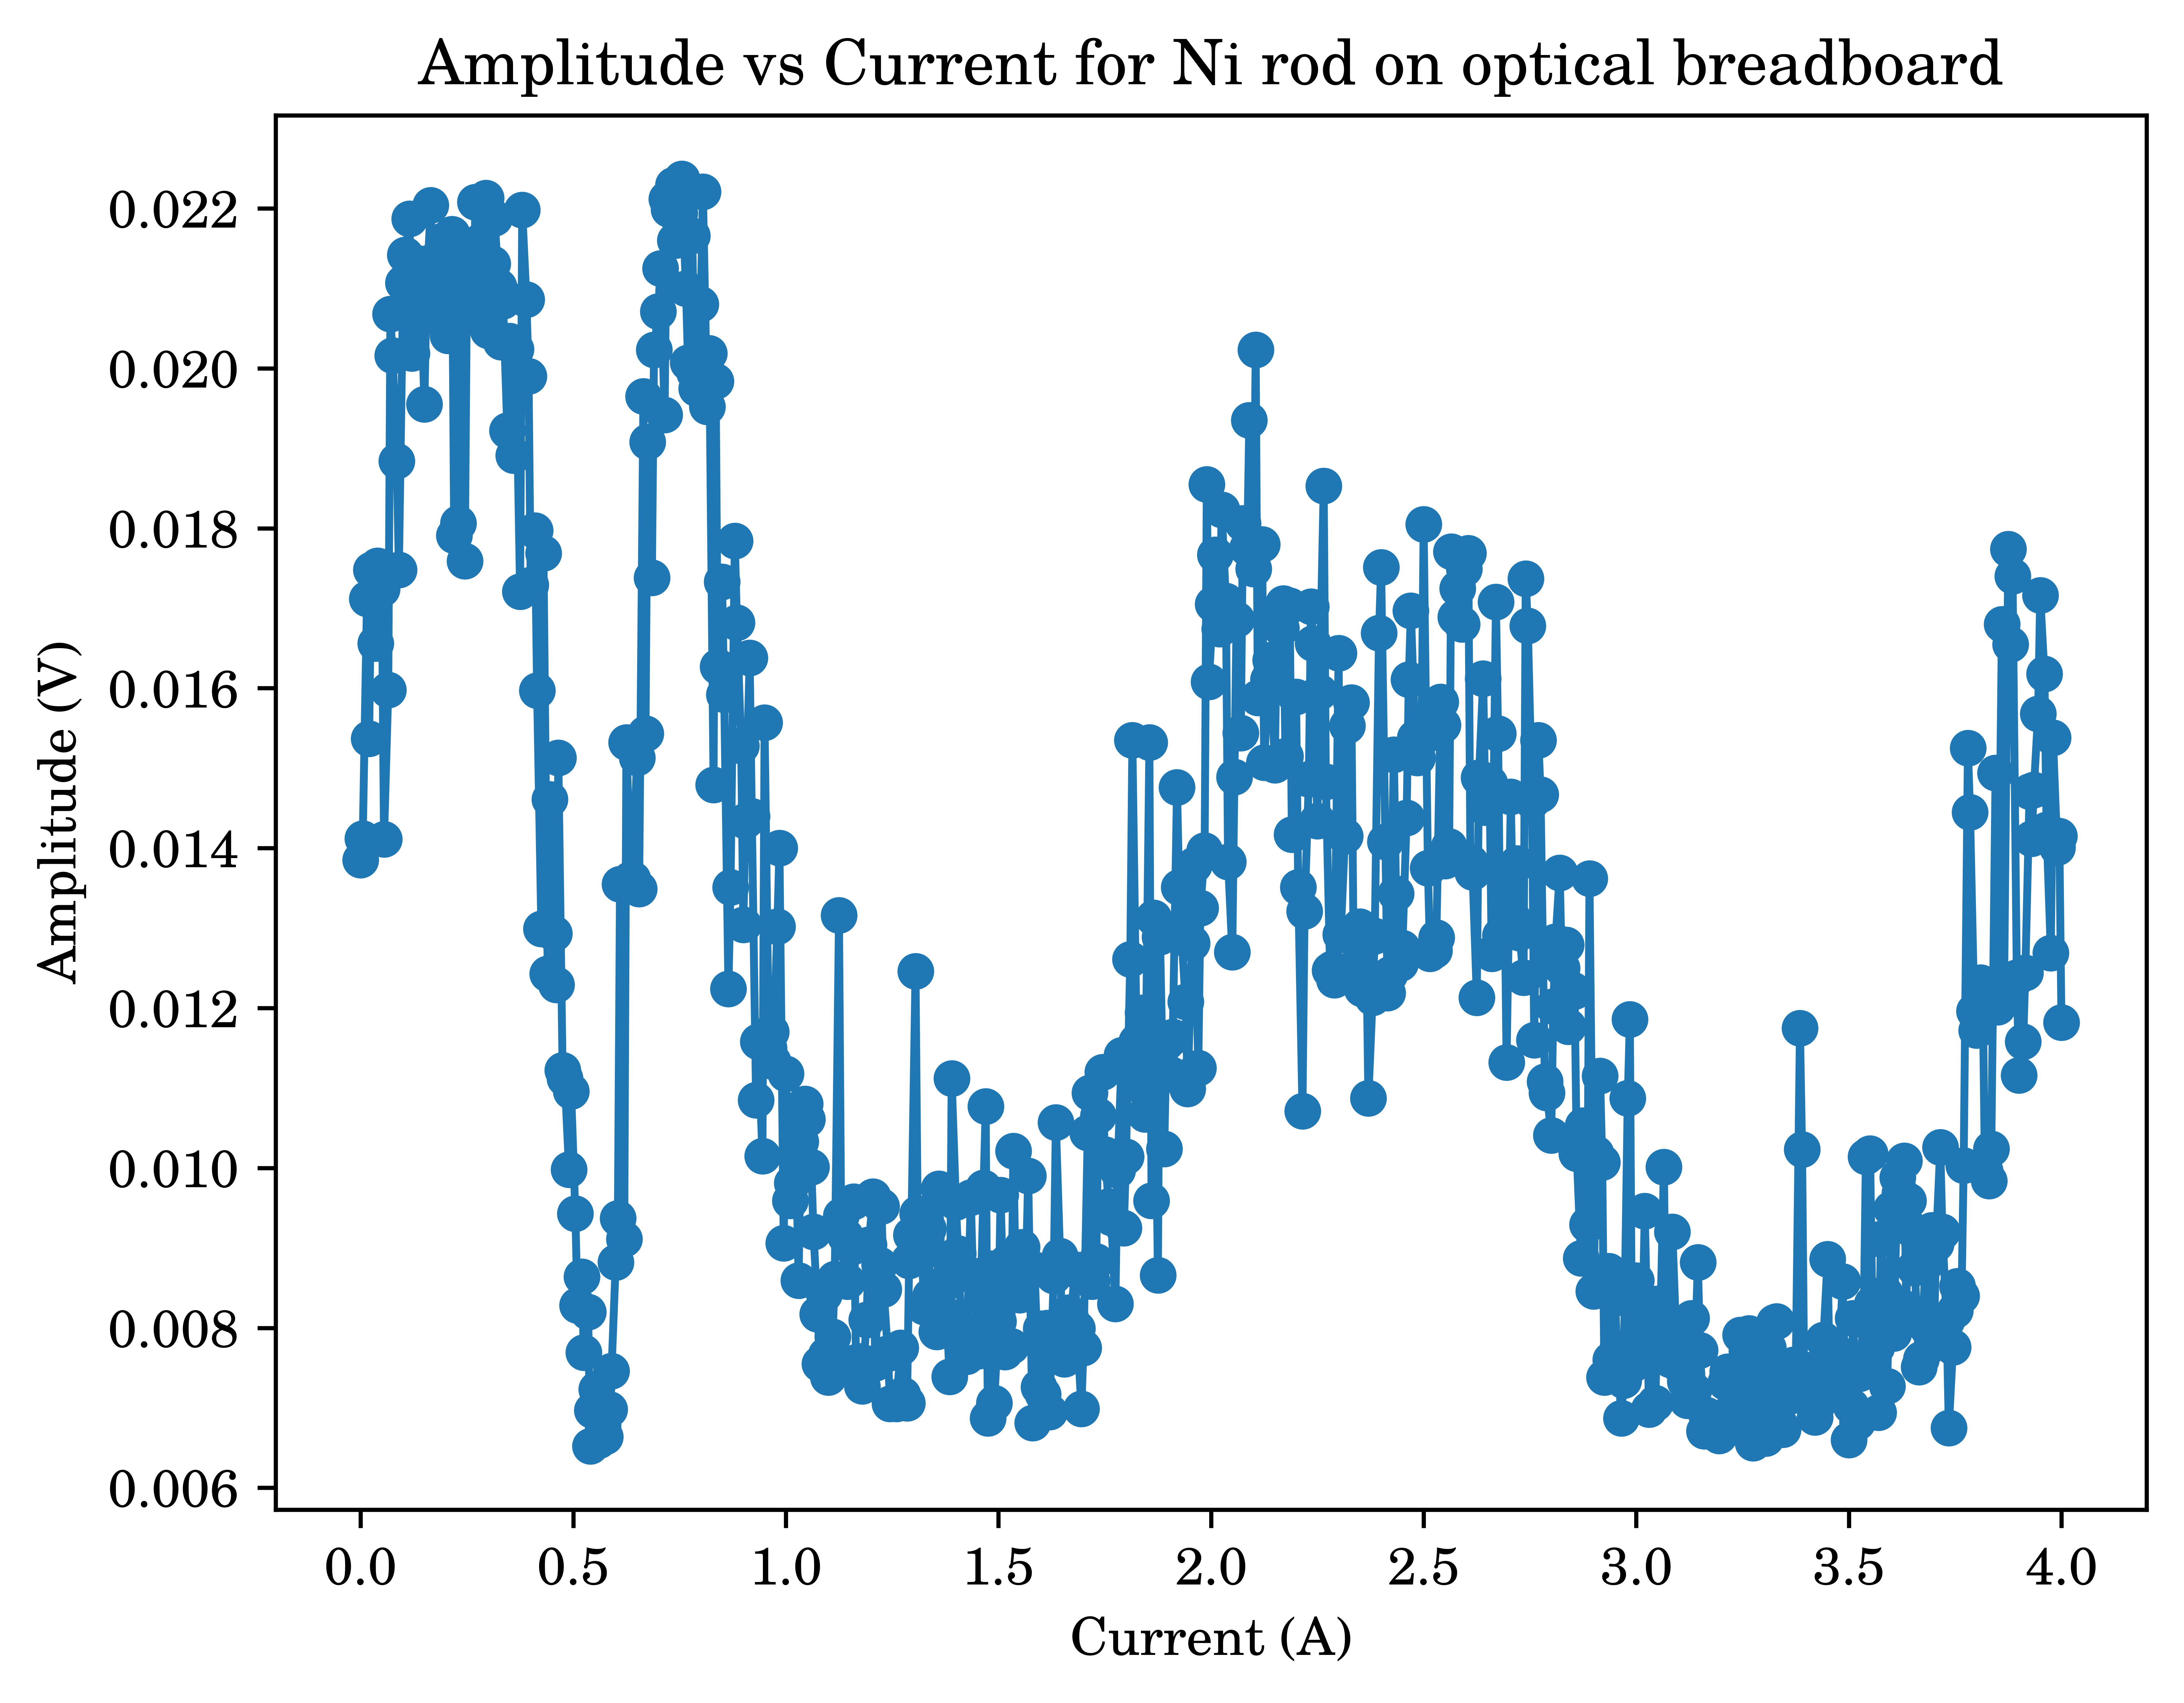
\includegraphics{data/ob-Fe-0}
	\caption{The amplitude versus current data obtained for Fe rod on the optical breadboard with altered arm lengths of the interferometer.}
	\label{fig:ob-fe-0}
\end{figure}

% Please add the following required packages to your document preamble:
% \usepackage{booktabs}
% \usepackage{graphicx}
\begin{table}[]
	\centering
	\resizebox{\textwidth}{!}{%
		\begin{tabular}{@{}ccccc@{}}
			\toprule
		\textbf{\begin{tabular}[c]{@{}c@{}}Current\\ (\si{\ampere})\end{tabular}} & \textbf{\begin{tabular}[c]{@{}c@{}}Ring changes\\ ($n$)\end{tabular}} & \textbf{\begin{tabular}[c]{@{}c@{}}$\Delta l$\\ ($\times 10^{-9} \si{\meter}$)\end{tabular}} & \textbf{\begin{tabular}[c]{@{}c@{}}Magnetization, $H$\\ ($\si{\ampere \per \meter}$)\end{tabular}} & \textbf{\begin{tabular}[c]{@{}c@{}}$\Delta l/l$\\ ($\times 10^{-9} \si{\meter}$)\end{tabular}} \\ \midrule
			0.46  & 2   & 3.16E-07 & 3.86E+03 & 2.21E-06 \\
			0.465 & 2.5 & 3.96E-07 & 3.90E+03 & 2.77E-06 \\
			0.49  & 3   & 4.75E-07 & 4.11E+03 & 3.32E-06 \\
			0.495 & 2.5 & 3.96E-07 & 4.15E+03 & 2.77E-06 \\
			0.51  & 2   & 3.16E-07 & 4.28E+03 & 2.21E-06 \\
			0.52  & 1.5 & 2.37E-07 & 4.36E+03 & 1.66E-06 \\
			0.525 & 1   & 1.58E-07 & 4.41E+03 & 1.11E-06 \\
			0.535 & 0.5 & 7.91E-08 & 4.49E+03 & 5.53E-07 \\
			0.54  & 0   & 0.00E+00 & 4.53E+03 & 0.00E+00 \\ \bottomrule
		\end{tabular}%
	}
	\caption{The variation in strain with applied magnetic field for Fe on the optical breadboard.}
	\label{tab:ob-Fe}
\end{table}
\begin{figure}
	\centering
	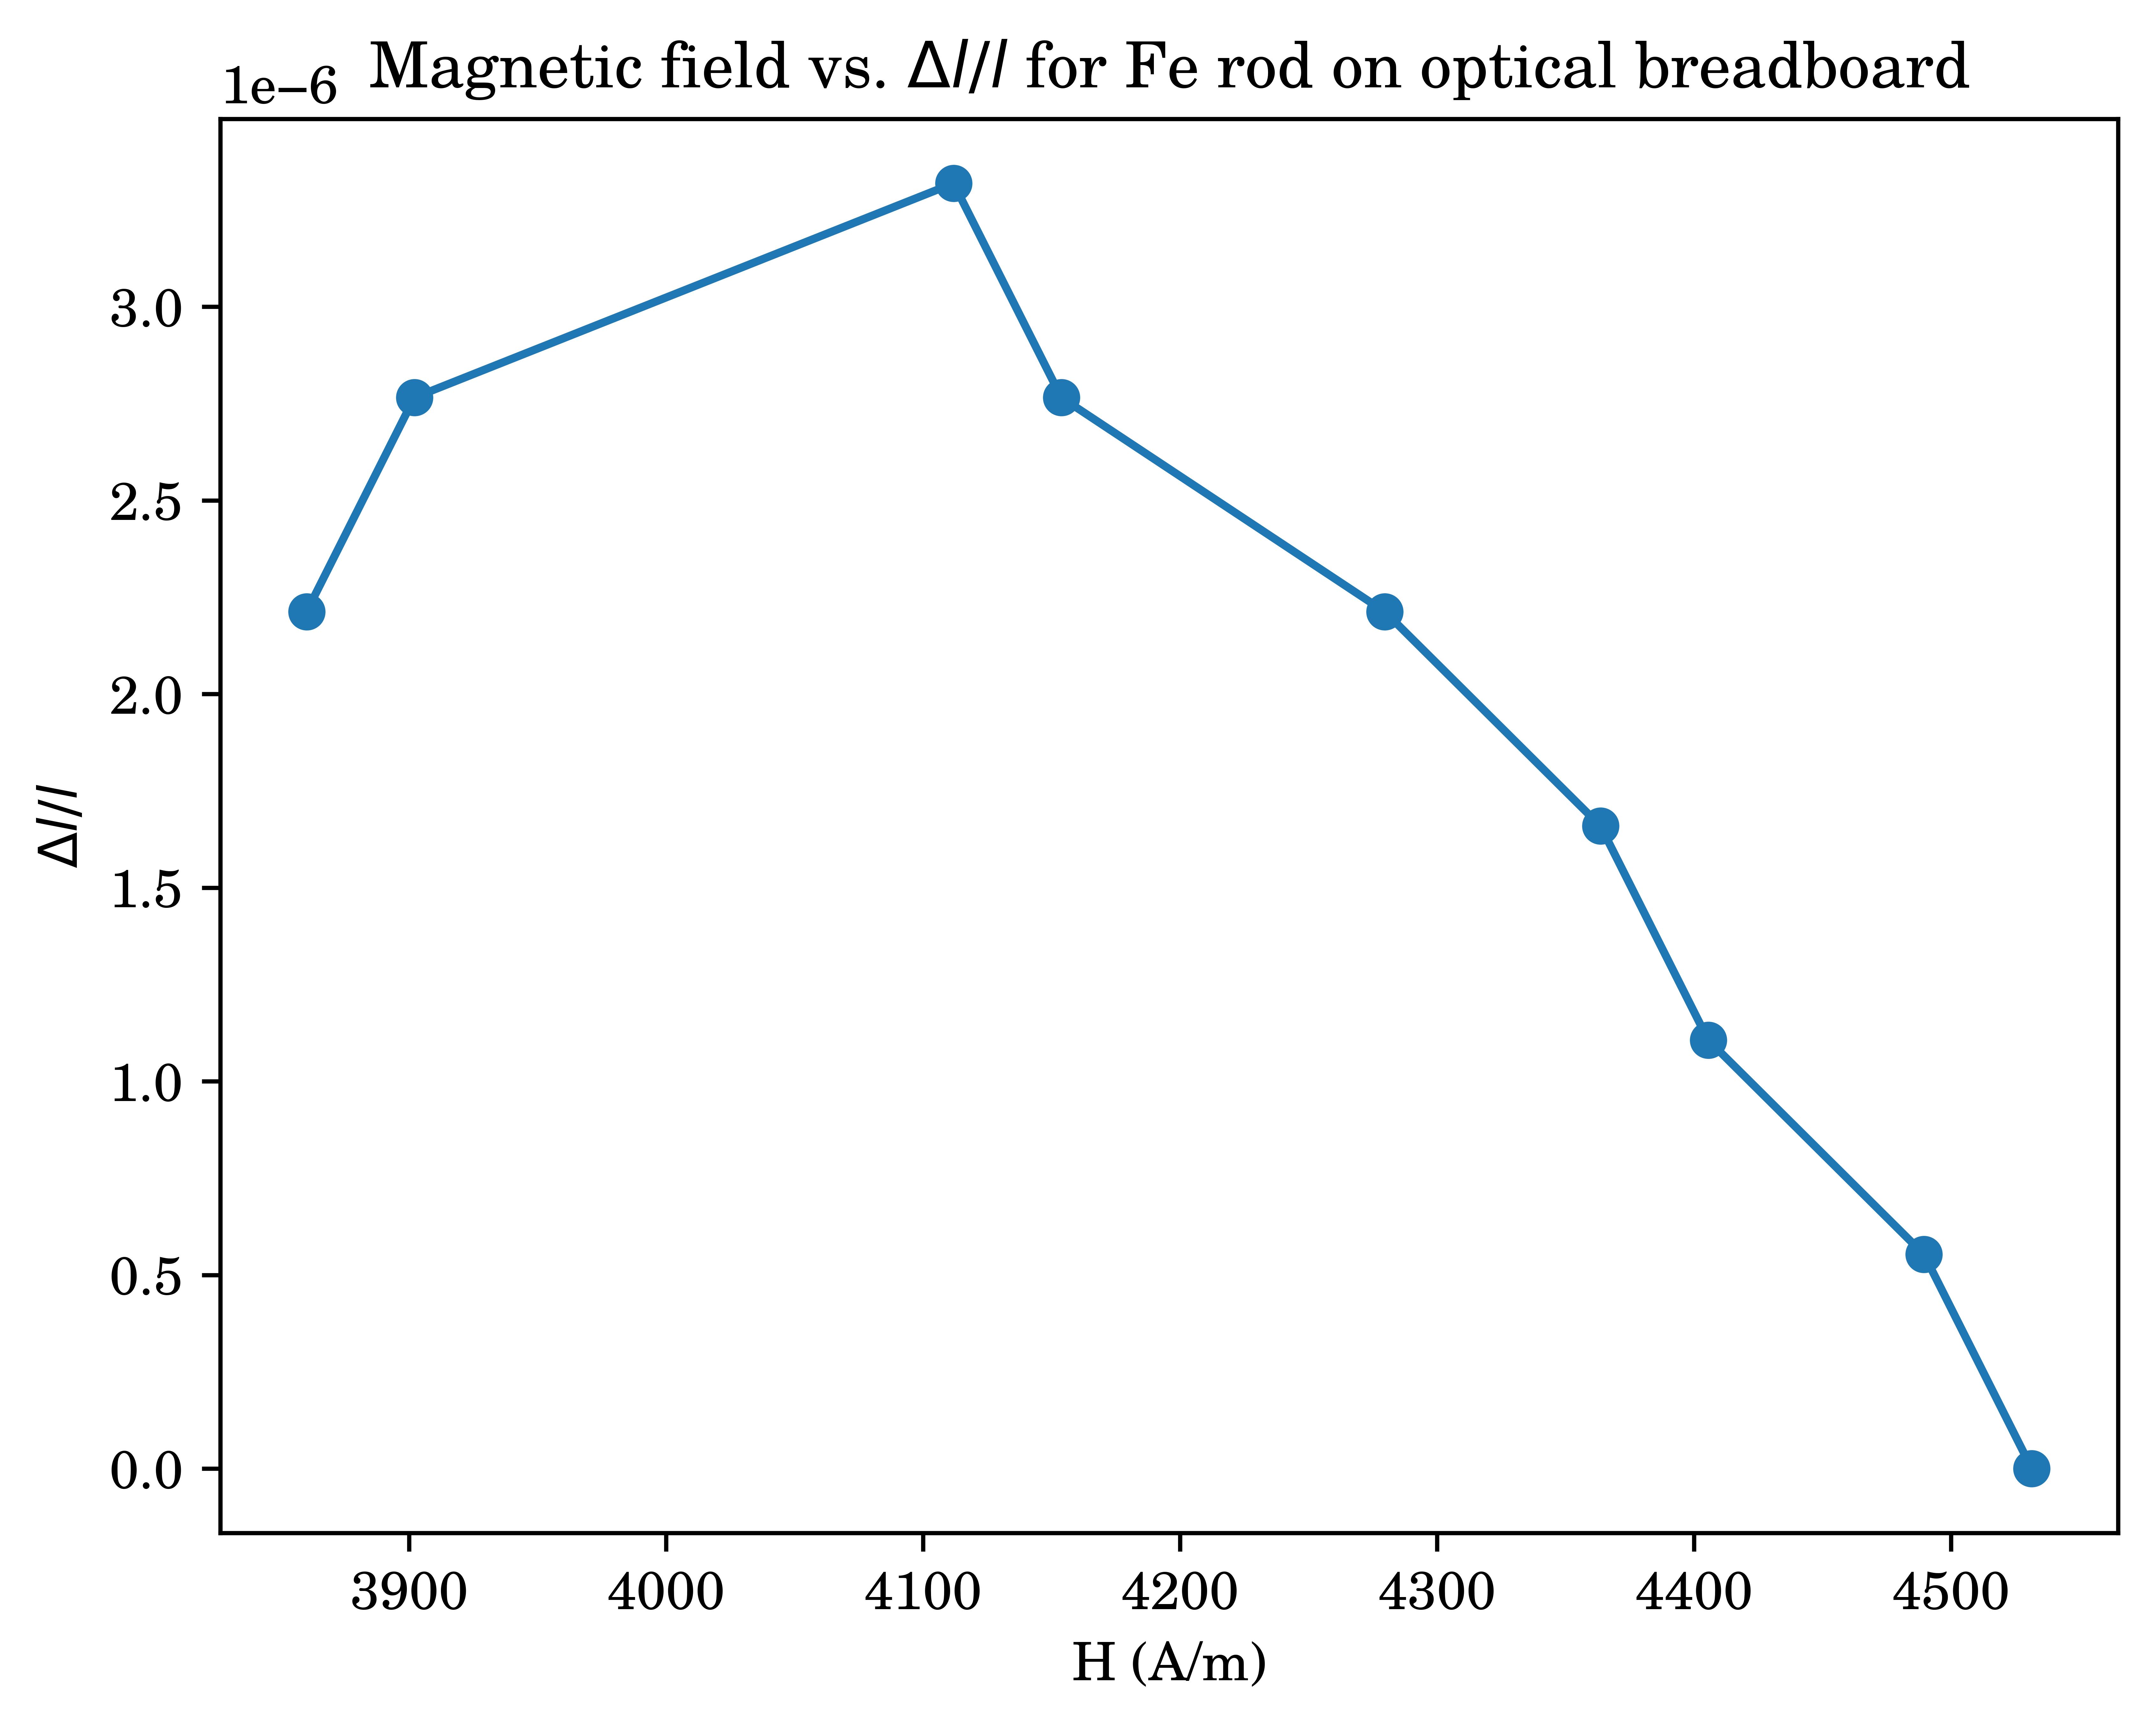
\includegraphics{data/ob-Fe-1}
	\caption{The variation in strain with applied magnetic field for Fe on the optical breadboard.}
	\label{fig:ob-fe-1}
\end{figure}

\section{With Nickel}
\begin{figure}
	\centering
	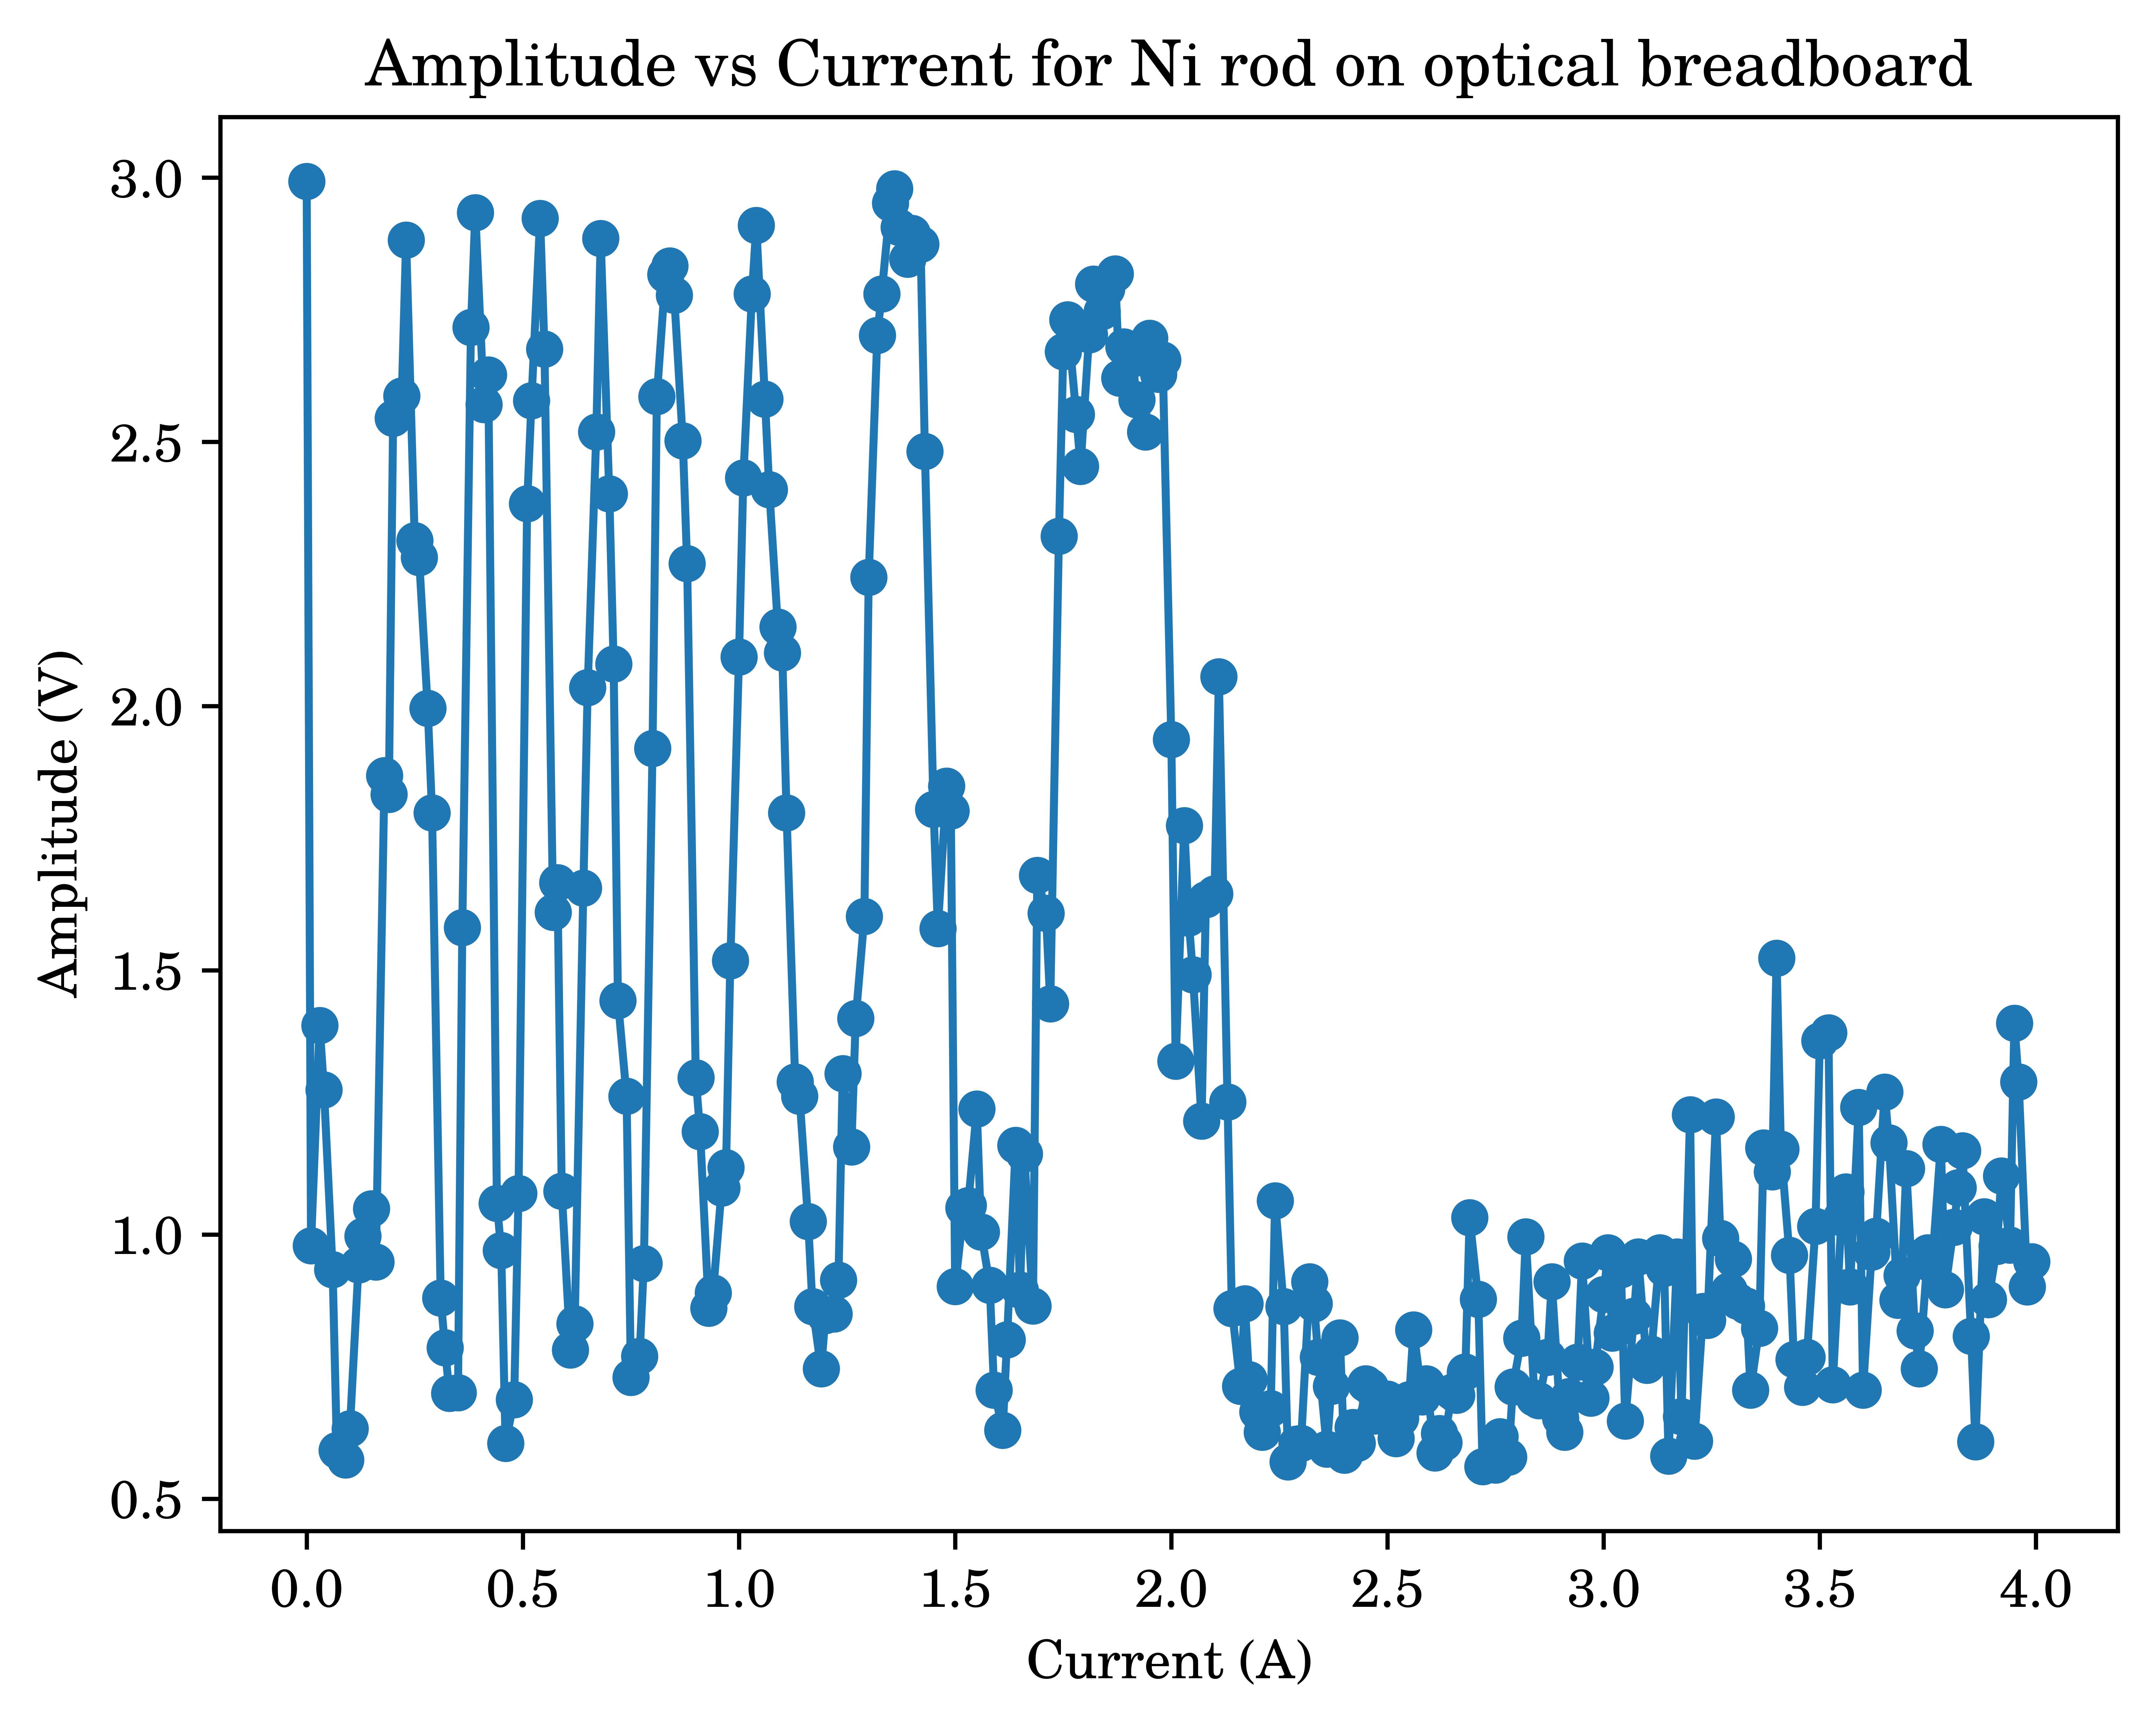
\includegraphics{data/ob-Ni-0}
	\caption{The amplitude versus current data obtained for Ni rod on the optical breadboard with altered arm lengths of the interferometer.}
	\label{fig:ob-ni-0}
\end{figure}

% Please add the following required packages to your document preamble:
% \usepackage{booktabs}
% \usepackage{graphicx}
\begin{table}[]
	\centering
	\resizebox{\textwidth}{!}{%
		\begin{tabular}{@{}ccccc@{}}
			\toprule
			\textbf{\begin{tabular}[c]{@{}c@{}}Current\\ (\si{\ampere})\end{tabular}} & \textbf{\begin{tabular}[c]{@{}c@{}}Ring changes\\ ($n$)\end{tabular}} & \textbf{\begin{tabular}[c]{@{}c@{}}$\Delta l$\\ ($\times 10^{-9} \si{\meter}$)\end{tabular}} & \textbf{\begin{tabular}[c]{@{}c@{}}Magnetization, $H$\\ ($\si{\ampere \per \meter}$)\end{tabular}} & \textbf{\begin{tabular}[c]{@{}c@{}}$\Delta l/l$\\ ($\times 10^{-9} \si{\meter}$)\end{tabular}} \\ \midrule
			0.01 & 0.5  & -7.91E-08 & 8.39E+01 & -5.53E-07 \\
			0.03 & 1    & -1.58E-07 & 2.52E+02 & -1.11E-06 \\
			0.09 & 1.5  & -2.37E-07 & 7.55E+02 & -1.66E-06 \\
			0.15 & 2    & -3.16E-07 & 1.26E+03 & -2.21E-06 \\
			0.16 & 2.5  & -3.96E-07 & 1.34E+03 & -2.77E-06 \\
			0.18 & 3    & -4.75E-07 & 1.51E+03 & -3.32E-06 \\
			0.19 & 3.5  & -5.54E-07 & 1.59E+03 & -3.87E-06 \\
			0.23 & 4    & -6.33E-07 & 1.93E+03 & -4.43E-06 \\
			0.33 & 4.5  & -7.12E-07 & 2.77E+03 & -4.98E-06 \\
			0.39 & 5    & -7.91E-07 & 3.27E+03 & -5.53E-06 \\
			0.41 & 5.5  & -8.70E-07 & 3.44E+03 & -6.08E-06 \\
			0.42 & 6    & -9.49E-07 & 3.52E+03 & -6.64E-06 \\
			0.46 & 6.5  & -1.03E-06 & 3.86E+03 & -7.19E-06 \\
			0.54 & 7    & -1.11E-06 & 4.53E+03 & -7.74E-06 \\
			0.57 & 7.5  & -1.19E-06 & 4.78E+03 & -8.30E-06 \\
			0.58 & 8    & -1.27E-06 & 4.87E+03 & -8.85E-06 \\
			0.61 & 8.5  & -1.34E-06 & 5.12E+03 & -9.40E-06 \\
			0.68 & 9    & -1.42E-06 & 5.71E+03 & -9.96E-06 \\
			0.75 & 9.5  & -1.50E-06 & 6.29E+03 & -1.05E-05 \\
			0.84 & 10   & -1.58E-06 & 7.05E+03 & -1.11E-05 \\
			0.93 & 10.5 & -1.66E-06 & 7.80E+03 & -1.16E-05 \\
			1.04 & 11   & -1.74E-06 & 8.73E+03 & -1.22E-05 \\
			1.19 & 11.5 & -1.82E-06 & 9.99E+03 & -1.27E-05 \\
			1.24 & 12   & -1.90E-06 & 1.04E+04 & -1.33E-05 \\
			1.26 & 12.5 & -1.98E-06 & 1.06E+04 & -1.38E-05 \\
			1.36 & 13   & -2.06E-06 & 1.14E+04 & -1.44E-05 \\
			1.39 & 13.5 & -2.14E-06 & 1.17E+04 & -1.49E-05 \\
			1.4  & 14   & -2.21E-06 & 1.17E+04 & -1.55E-05 \\
			1.46 & 14.5 & -2.29E-06 & 1.23E+04 & -1.60E-05 \\
			1.48 & 15   & -2.37E-06 & 1.24E+04 & -1.66E-05 \\ \bottomrule
		\end{tabular}%
	}
	\caption{The variation in strain with applied magnetic field for Ni on the optical breadboard.}
	\label{tab:ob-Ni}
\end{table}
\begin{figure}
	\centering
	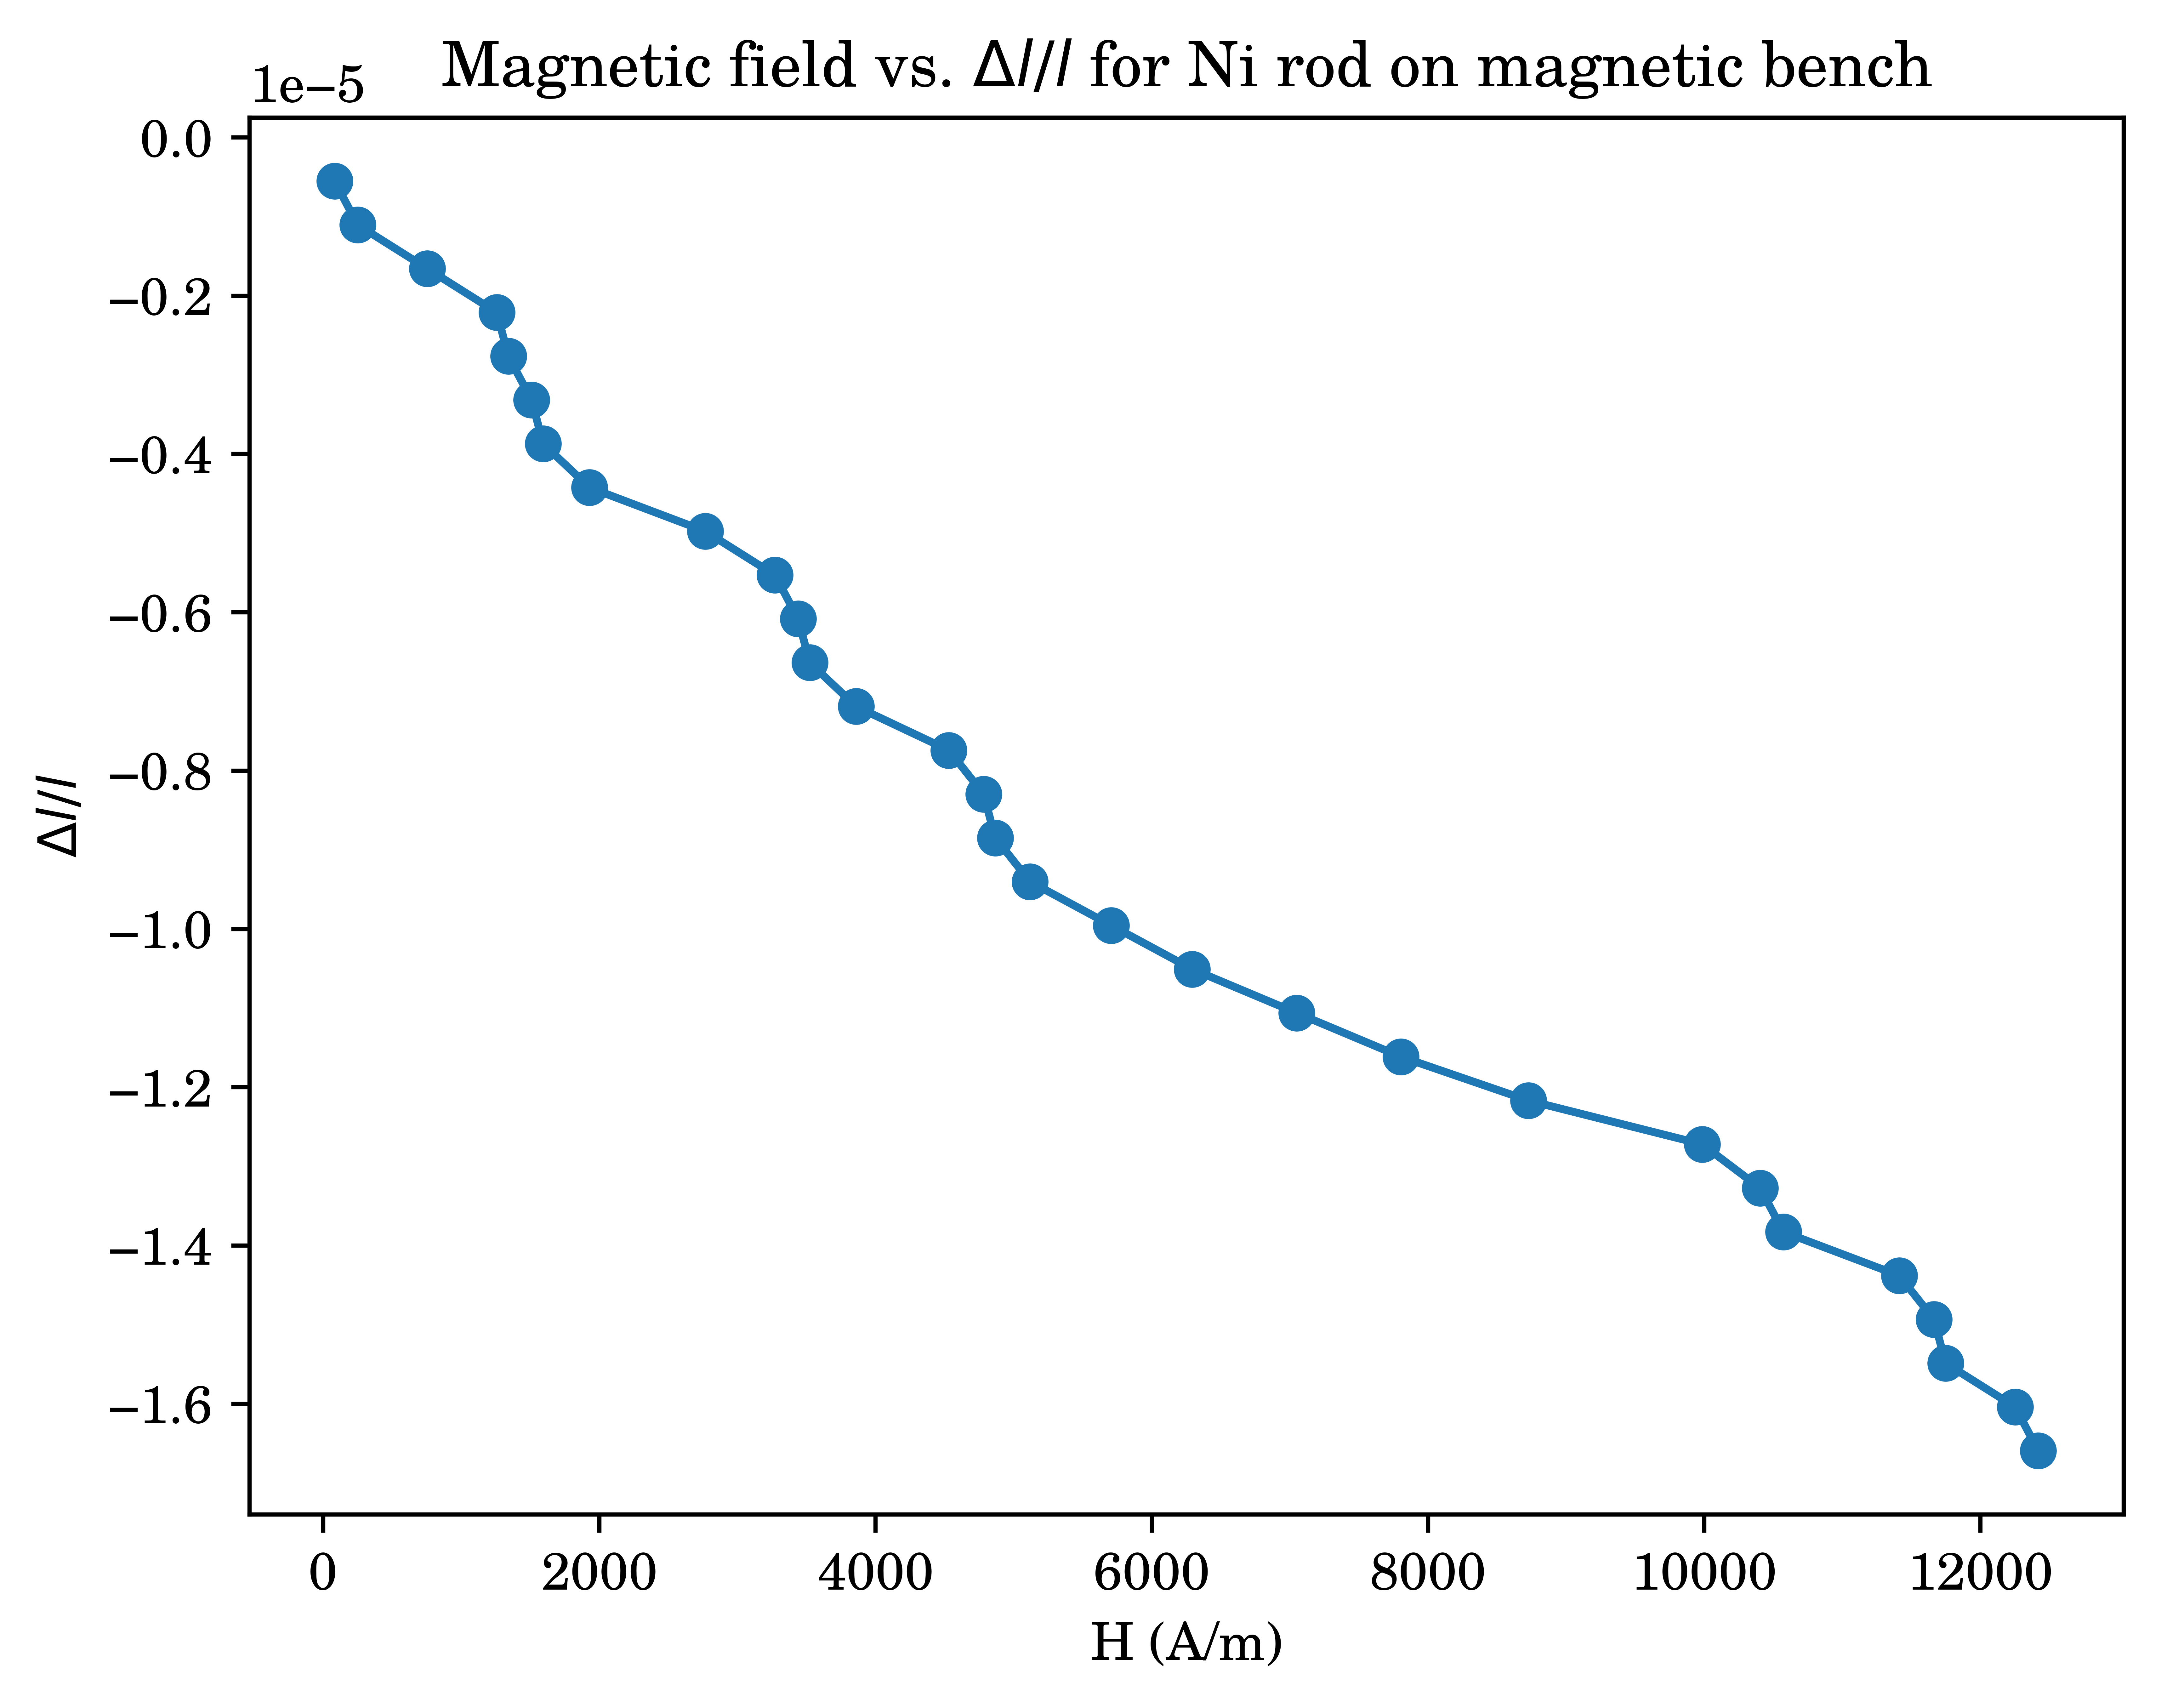
\includegraphics{data/ob-Ni-1}
	\caption{The variation in strain with applied magnetic field for Ni on the optical breadboard.}
	\label{fig:ob-ni-1}
\end{figure}

\setcounter{equation}{0}
\setcounter{table}{0}
\setcounter{figure}{0}